\documentclass[10pt,twocolumn,twoside,]{pinp}

%% Some pieces required from the pandoc template
\providecommand{\tightlist}{%
  \setlength{\itemsep}{0pt}\setlength{\parskip}{0pt}}

% Use the lineno option to display guide line numbers if required.
% Note that the use of elements such as single-column equations
% may affect the guide line number alignment.

\usepackage[T1]{fontenc}
\usepackage[utf8]{inputenc}

% pinp change: the geometry package layout settings need to be set here, not in pinp.cls
\geometry{layoutsize={0.95588\paperwidth,0.98864\paperheight},%
  layouthoffset=0.02206\paperwidth, layoutvoffset=0.00568\paperheight}

\definecolor{pinpblue}{HTML}{185FAF}  % imagecolorpicker on blue for new R logo
\definecolor{pnasbluetext}{RGB}{101,0,0} %


\usepackage[version = 4]{mhchem}
\usepackage{booktabs}
\usepackage{longtable}
\usepackage{array}
\usepackage{multirow}
\usepackage{wrapfig}
\usepackage{float}
\usepackage{colortbl}
\usepackage{pdflscape}
\usepackage{tabu}
\usepackage{threeparttable}
\usepackage{threeparttablex}
\usepackage[normalem]{ulem}
\usepackage{makecell}
\usepackage{xcolor}

\title{An Introduction to PCA}

\author[a]{Bryan A. Hanson}

  \affil[a]{Prof.~Emeritus, Dept. of Chemistry \& Biochemistry, DePauw
University; \url{hanson@depauw.edu}}

\setcounter{secnumdepth}{0}

% Please give the surname of the lead author for the running footer
\leadauthor{}

% Keywords are not mandatory, but authors are strongly encouraged to provide them. If provided, please include two to five keywords, separated by the pipe symbol, e.g:
 

\begin{abstract}

\end{abstract}

\dates{This version was compiled on \today} 

% initially we use doi so keep for backwards compatibility
% new name is doi_footer

\pinpfootercontents{Intro to PCA}

\begin{document}

% Optional adjustment to line up main text (after abstract) of first page with line numbers, when using both lineno and twocolumn options.
% You should only change this length when you've finalised the article contents.
\verticaladjustment{-2pt}

\maketitle
\thispagestyle{firststyle}
\ifthenelse{\boolean{shortarticle}}{\ifthenelse{\boolean{singlecolumn}}{\abscontentformatted}{\abscontent}}{}

% If your first paragraph (i.e. with the \dropcap) contains a list environment (quote, quotation, theorem, definition, enumerate, itemize...), the line after the list may have some extra indentation. If this is the case, add \parshape=0 to the end of the list environment.


The audience for this document is chemists, spectroscopists and people
in allied fields who are using spectroscopy to analyze their data.

We will use two data sets here: one is a set of elemental analyses of
glass artifacts; we use this relatively small, non-spectroscopic data
set to help understand PCA fundamentals. The second data set is a
collection of IR spectra of plant oils.

\hypertarget{conceptual-introduction-to-pca}{%
\section{Conceptual Introduction to
PCA}\label{conceptual-introduction-to-pca}}

PCA is conducted on data sets composed of:

\begin{itemize}
\tightlist
\item
  Samples, typically in rows.
\item
  Variables which were measured for each sample.
\end{itemize}

The purpose of PCA is \emph{data reduction}. This term refers to the
goal of:

\begin{itemize}
\tightlist
\item
  Reducing the size of the data set by identifying variables that are
  not informative. Such variables are also described as ``noisy'', in
  that they don't add anything to the study. Such variables arise
  naturally in many situations. Example: a survey about food preferences
  may include questions about political party. The answers about
  political party may not be informative.
\item
  Collapsing correlating variables. Several of the variables measured in
  a study may actually be measures of the same underlying reality. This
  is not to say they are noisy, but rather they may be redundant.
  Example: a survey asks participants if they eat kale, and separately,
  if they eat quinoa. Individuals may answer yes to both questions or no
  to both questions. The answers may reflect the individuals preference
  for a healthy diet. Either question alone may be sufficient. PCA will
  collapse these correlating variables into one variable.
\end{itemize}

What does one get from PCA?

\begin{itemize}
\tightlist
\item
  An indication of how many principal components (PC) are needed to
  describe the data, generally presented as a \emph{scree plot}.
\item
  Scores, generally presented as one or more \emph{score plots}.
\item
  Loadings, generally presented as one or more \emph{loading plots}.
\end{itemize}

These plots will be explained further in the next section. Other things
to know about PCA before going further:

\begin{itemize}
\tightlist
\item
  PCA is \emph{principal} not \emph{principle} components analysis!
\item
  PCA is the ``mother'' of a number of other related techniques, so if
  you plan further study it is critical to understand PCA to the
  greatest degree possible.
\item
  That said, it takes most people a long time to fully grasp what PCA
  does, especially from the mathematical perspective. Don't expect to
  get all the nuances on the first pass!
\item
  \emph{And the problem} \ldots The results of PCA, scores and loadings,
  exist in a so-called abstract space. This space is only distantly and
  indirectly related to the space in which the original samples reside.
  Therefore, the results of PCA are frequently difficult to interepret
  in concrete terms. See previous point.
\end{itemize}

\hypertarget{pca-results-illustrated-no-code-no-math}{%
\section{PCA Results Illustrated, No Code, No
Math}\label{pca-results-illustrated-no-code-no-math}}

This section is designed to illustrate the concepts of PCA, and how to
interpret the plots that arise from PCA.

We'll use a data set which reports chemical analyses on archaeological
glass artifacts that was designed to determine the origin of the
artifacts. Table \ref{tab:dataTaste} gives a little bit of the data
set.\footnote{This is the \code{glass} data set in package \code{chemometrics}.}

\begin{table}

\caption{\label{tab:dataTaste}A portion of the archaeological glass data set. Values are percentages.\label{tab:dataTaste}}
\centering
\begin{tabular}[t]{r|r|r|r|r|r|r|r}
\hline
Na2O & MgO & Al2O3 & SiO2 & P2O5 & SO3 & Cl & K2O\\
\hline
13.904 & 2.244 & 1.312 & 67.752 & 0.884 & 0.052 & 0.936 & 3.044\\
\hline
14.194 & 2.184 & 1.310 & 67.076 & 0.938 & 0.024 & 0.966 & 3.396\\
\hline
14.668 & 3.034 & 1.362 & 63.254 & 0.988 & 0.064 & 0.886 & 2.828\\
\hline
14.800 & 2.455 & 1.385 & 63.790 & 1.200 & 0.115 & 0.988 & 2.878\\
\hline
14.078 & 2.480 & 1.072 & 68.768 & 0.682 & 0.070 & 0.966 & 2.402\\
\hline
\end{tabular}
\end{table}

There are 180 glass artifacts (the samples) in this data set (hence 180
rows), and the elements analyzed were \ce{Na2O}, \ce{MgO}, \ce{Al2O3},
\ce{SiO2}, \ce{P2O5}, \ce{SO3}, \ce{Cl}, \ce{K2O}, \ce{CaO}, \ce{MnO},
\ce{Fe2O3}, \ce{BaO}, and \ce{PbO}
.\footnote{The elements are reported as their oxides in the form of weight percent.}

We'll perform PCA on the glass data set, show the three plots and then
discuss them in turn. Figure \ref{fig:glassScree} shows the scree plot,
Figure \ref{fig:glassScores} shows the score plot and Figure
\ref{fig:glassLoadings} shows the first loadings.

\begin{figure}

{\centering 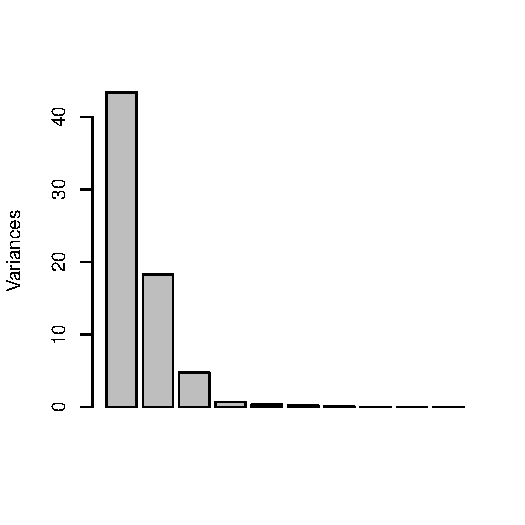
\includegraphics{/Users/bryanhanson/Documents/Professional/Research/R_Pkgs/ChemoSpec/docs/articles/IntroPCA_files/figure-latex/glassScree-1} 

}

\caption{Scree plot from PCA on the glass data set.\label{fig:glassScree}}\label{fig:glassScree}
\end{figure}

Figure \ref{fig:glassScree}, the scree plot, shows the amount of
variance in the data set explained by each principal component (PCs are
along the x axis, from 1 to
10).\footnote{Because there are 13 variables, the most PCs one could have is 13.  In theory, keeping all 13 PCs perfectly reproduces the original data set.}
For now, think of variance as the variation or variability in the data
set, or better, think of it as the hidden signal in the data. To
interpret this plot, we look for the point at which the height of the
bars suddenly levels off. In this case, the first three PCs drop
steadily downward, but from PC four and onward there is little
additional variation (signal) that can be explained. We would say that
three PCs are enough to explain this data set. In other words, the
original 13 variables have been reduced to three, which is a great
simplification.

\begin{figure}

{\centering 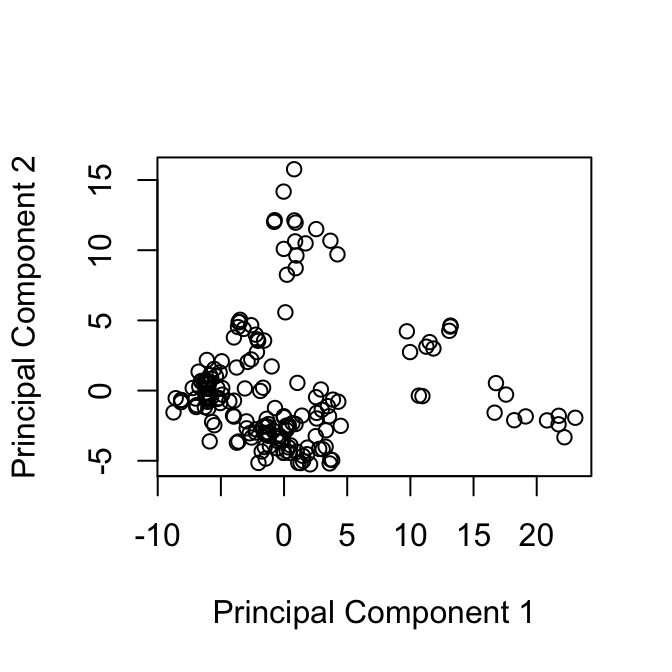
\includegraphics{/Users/bryanhanson/Documents/Professional/Research/R_Pkgs/ChemoSpec/docs/articles/IntroPCA_files/figure-latex/glassScores-1} 

}

\caption{Score plot from PCA on the glass data set.\label{fig:glassScores}}\label{fig:glassScores}
\end{figure}

In Figure \ref{fig:glassScores} one sees the scores for PC 1 plotted
against the scores for PC 2. There are 180 points in this plot because
there is one point per sample (put another way, every sample has a score
value for PC 1 and for PC 2). This plot is interpreted by looking for
clustering of samples, as well as for samples that are outliers, off by
themselves. Depending upon your eye, there are 3 to 5 clusters here.
Later we'll discuss how we can explore this further.

We could also plot PC 1 against PC 3, or PC 2 against PC 3. These might
show different clustering and separation of samples, but are not shown
here. There wouldn't be much point in plotting PC 4 or higher, as PCs 4
and higher are mostly noise, not signal, as established by the scree
plot (Figure \ref{fig:glassScree}).

\begin{figure}

{\centering 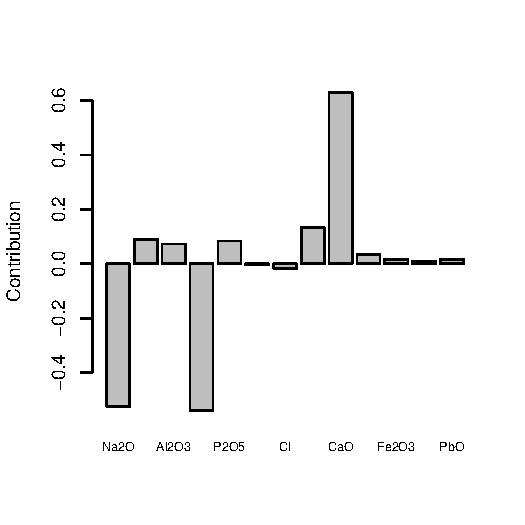
\includegraphics{/Users/bryanhanson/Documents/Professional/Research/R_Pkgs/ChemoSpec/docs/articles/IntroPCA_files/figure-latex/glassLoadings-1} 

}

\caption{Loadings plot for the first PC from PCA on the glass data set.\label{fig:glassLoadings}}\label{fig:glassLoadings}
\end{figure}

The loadings plot, Figure \ref{fig:glassLoadings}, shows how much each
measured variable contributes to the component and hence the separation
of samples (in this case the loadings for PC 1). We see that three
elements have large loadings, and the other elements contribute little
to the separation. We would say separation along PC 1 is driven largely
and \emph{collectively} by the results for \ce{Na2O}, \ce{SiO2} and
\ce{CaO}.\footnote{If you knew this would be the result ahead of time, you probably would not have taken the time and expense to analyze the uninformative elements.  However, we haven't looked at PC 2 or PC 3 so this conclusion is premature.}
The first PC should be interpreted as a composite of these variables --
these variables have been collapsed into one new variable, PC 1.

\hypertarget{refinements-1}{%
\subsection{Refinements 1}\label{refinements-1}}

Rather than relying on a scree plot to determine the number of PCs that
are important, we can present the same information in a table, see Table
\ref{tab:screeTable}. A general rule of thumb says to keep enough PCs to
account for 95\% of the variation (signal). The table tells us the same
as the plot: keep three PCs.

\begin{table}

\caption{\label{tab:screeTable}Variance (signal) accounted for by PCs. Values in percent.\label{tab:screeTable}}
\centering
\begin{tabular}[t]{l|r|r}
\hline
component & variance & cumulative\\
\hline
PC 1 & 64 & 64\\
\hline
PC 2 & 27 & 91\\
\hline
PC 3 & 7 & 98\\
\hline
PC 4 & 1 & 99\\
\hline
PC 5 & 0 & 100\\
\hline
PC 6 & 0 & 100\\
\hline
PC 7 & 0 & 100\\
\hline
PC 8 & 0 & 100\\
\hline
PC 9 & 0 & 100\\
\hline
PC 10 & 0 & 100\\
\hline
PC 11 & 0 & 100\\
\hline
PC 12 & 0 & 100\\
\hline
PC 13 & 0 & 100\\
\hline
\end{tabular}
\end{table}

\hypertarget{refinements-2}{%
\subsection{Refinements 2}\label{refinements-2}}

The mathematics of PCA do not take into account anything about the
samples other than the measured variables. However, the researcher may
well know something about the samples, for instance, they may fall into
groups based on their origin. If this is the case, the points on the
score plot can be colored according to the group. This may aid
significantly in the interpretation. Lucky for us, we can do this for
the glass data set. The samples fell into four groups. We'll re-do the
score plot with colors corresponding to the known groups (Figure
\ref{fig:glassScores2}).

\begin{figure}

{\centering 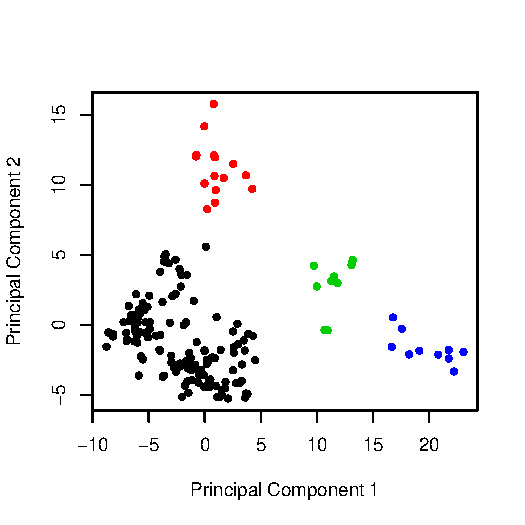
\includegraphics{/Users/bryanhanson/Documents/Professional/Research/R_Pkgs/ChemoSpec/docs/articles/IntroPCA_files/figure-latex/groups-1} 

}

\caption{Score plot from PCA on the glass data set, with groups color-coded.\label{fig:glassScores2}}\label{fig:groups}
\end{figure}

With this figure, we can see that the large group in the lower left
corner (in black), which to the eye might have been two groups, is
composed of related samples.

\hypertarget{a-spectroscopic-data-set}{%
\section{A Spectroscopic Data Set}\label{a-spectroscopic-data-set}}

The archaeological data set has the advantage of only having a few
variables, the percentages of each element in the glass artifacts. If we
move to a spectroscopic data set, the number of variables goes up
dramatically. A UV-Vis data set typically would have a few hundred to a
thousand wavelength variables, an IR data set perhaps a few thousand
data points, and a 1D NMR data set would typically have 16K or more data
points. As far as PCA is concerned, in these cases the scree plot and
score plot do not change in appearance or interpretation.

However, the loading plot changes appearance dramatically. This is
because with hundreds to thousands of variables, one would not create a
loading plot based on a bar chart (Figure \ref{fig:glassLoadings} is a
bar chart). Instead, the loading plot with many variables looks like a
spectrum! While the appearance is different, the interpretation is the
same as for when there are only a few variables.

Let's illustrate with an IR data set. We'll use a data set included with
the \code{ChemoSpec} package. This is a set of IR spectra of plant oils
which are mixtures of triglycerides (triacylglyerols, which are esters),
and free fatty acids. Figure \ref{fig:IRSpectrum} shows a typical
spectrum from the data
set.\footnote{Plots in this vignette are deliberately made rather plain to focus on the data and to be consistent for ease-of-comparison.  Package \code{ChemoSpec} makes much more polished plots.}

\begin{figure}

{\centering 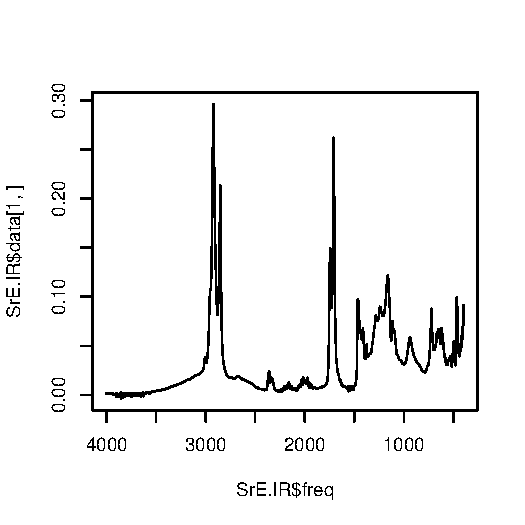
\includegraphics{/Users/bryanhanson/Documents/Professional/Research/R_Pkgs/ChemoSpec/docs/articles/IntroPCA_files/figure-latex/IRSpectrum-1} 

}

\caption{Spectrum 1 from the IR data set.\label{fig:IRSpecrum}}\label{fig:IRSpectrum}
\end{figure}

Next, we'll carry out PCA as before, and show the scree plot (Figure
\ref{fig:IRScree}) and the score plot (Figure \ref{fig:IRScores}). Note
that these appear like the corresponding plots for the glass data set,
and are interpreted in the same manner. However, the loadings plot,
Figure \ref{fig:IRLoadings}, looks a lot like a spectrum, because it has
1868 data points, and is plotted as a connected scatter plot and not as
a bar chart (which would be difficult to read).

\begin{figure}

{\centering 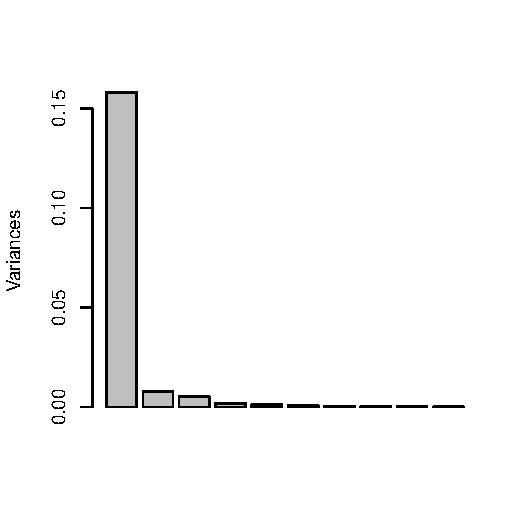
\includegraphics{/Users/bryanhanson/Documents/Professional/Research/R_Pkgs/ChemoSpec/docs/articles/IntroPCA_files/figure-latex/IRScree-1} 

}

\caption{Scree plot from PCA on the IR data set.\label{fig:IRScree}}\label{fig:IRScree}
\end{figure}

\begin{figure}

{\centering 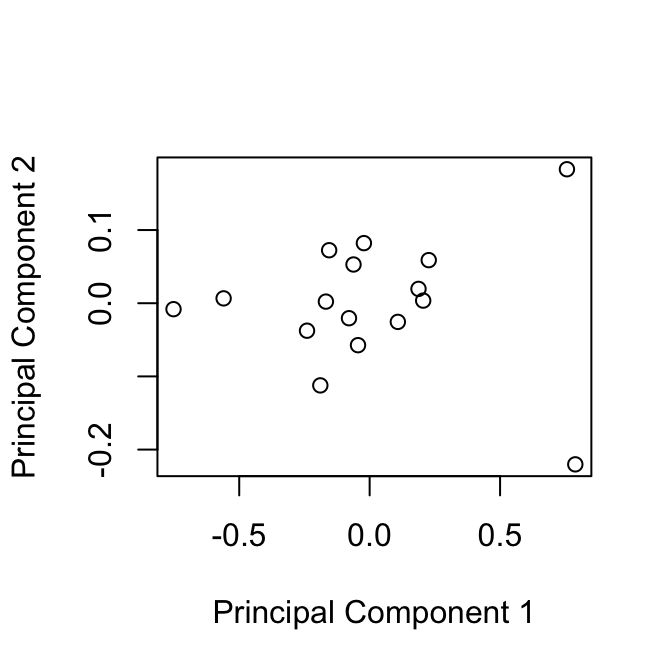
\includegraphics{/Users/bryanhanson/Documents/Professional/Research/R_Pkgs/ChemoSpec/docs/articles/IntroPCA_files/figure-latex/IRScores-1} 

}

\caption{Score plot from PCA on the IR data set.\label{fig:IRScores}}\label{fig:IRScores}
\end{figure}

\begin{figure}

{\centering 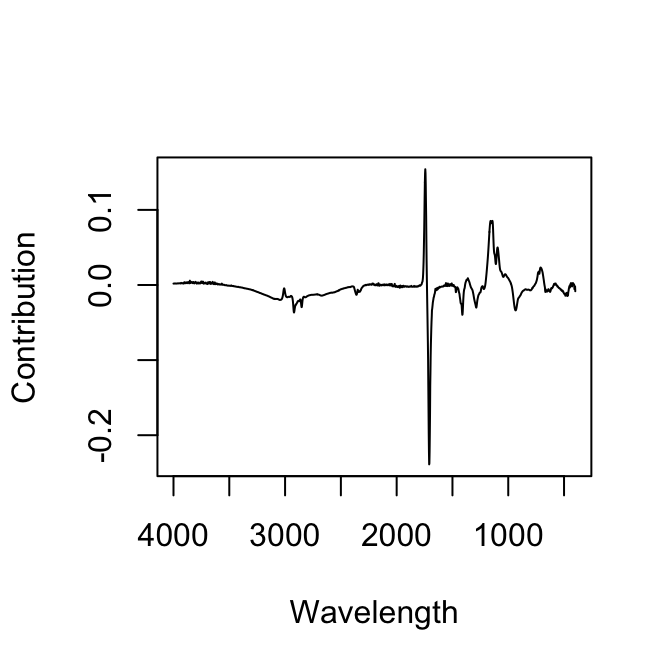
\includegraphics{/Users/bryanhanson/Documents/Professional/Research/R_Pkgs/ChemoSpec/docs/articles/IntroPCA_files/figure-latex/IRLoadings-1} 

}

\caption{Loadings plot for the first PC from PCA on the IR data set.\label{fig:IRLoadings}}\label{fig:IRLoadings}
\end{figure}

Let's look at the carbonyl region of the loadings plot in detail. Figure
\ref{fig:IRLoadings2} shows the original spectrum in red, for reference,
and the loadings in black. One can see that the ester carbonyl
contributes positively to the first loading, while the carboxylic acid
carbonyl contributes negatively.

Finally, to make the point that the loading plot for many variables is
essentially the same as the loading plot for just a few variables,
Figure \ref{fig:IRLoadings3} shows the carbonyl region as a kind of bar
plot. If one connects the tips of the bars together, one gets the
previous plot.

\begin{figure}

{\centering 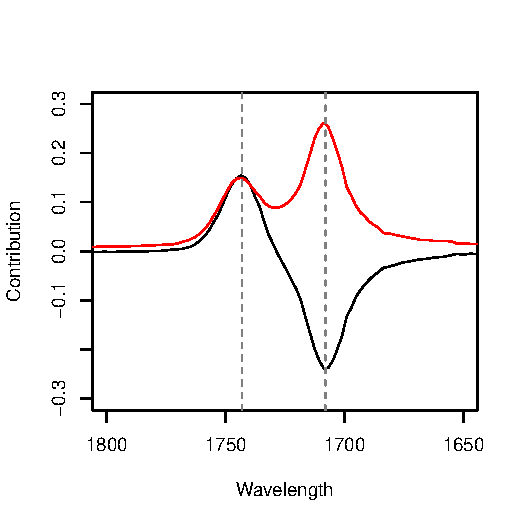
\includegraphics{/Users/bryanhanson/Documents/Professional/Research/R_Pkgs/ChemoSpec/docs/articles/IntroPCA_files/figure-latex/IRLoadings2-1} 

}

\caption{Loadings plot for the first PC from PCA on the IR data set, carbonyl region. Reference spectrum shown in red.\label{fig:IRLoadings2}}\label{fig:IRLoadings2}
\end{figure}

\begin{figure}

{\centering 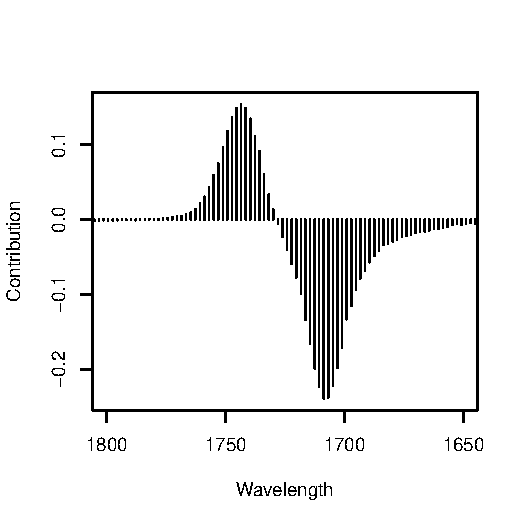
\includegraphics{/Users/bryanhanson/Documents/Professional/Research/R_Pkgs/ChemoSpec/docs/articles/IntroPCA_files/figure-latex/IRLoadings3-1} 

}

\caption{Loadings plot for the first PC from PCA on the IR data set, carbonyl region, shown as a bar plot.\label{fig:IRLoadings3}}\label{fig:IRLoadings3}
\end{figure}

%\showmatmethods





\end{document}
